\documentclass{article}

\usepackage{amsmath}
\usepackage{graphicx}

\def\pm{PYroMat}

\title{The ITER1 and HYBRID1 iteration algorithms used in the PYroMat package}
\author{Christopher R. Martin\\Assistant Professor of Mechanical Engineering\\Penn State University}
\date{\today}

\begin{document}

\maketitle

\section{Introduction}

In multi-phase substances, the general equation of state for the evaluation of thermodynamic properties of substances is almost always of the form, $A(T,\rho)$; the Helmholtz free energy expressed as a function of temperature and density.  Ideal gases are almost always defined in terms of $c_p(T)$; where $c_p$ is constant-pressure specific heat.  For an ideal gas, enthalpy and specific heats do not depend on pressure, but entropy's pressure dependency is straightforward, so ideal gas properties are usually evaluated in terms of temperature and pressure instead of temperature and density.

In general, all of the substances modeled by \pm may be thought of as having properties that are a function of any two of $T$, $p$, and $\rho$.  As of version 2.1.0, virtually all property methods in \pm accept any two of these three as a constraint on the substance state.  For two-phase mixtures (which are possible in the multi-phase collection) ``quality'' or $x$ may be specified instead of one of these.

The underlying models on which \pm is based permit relatively straightforward algorithms for calculating properties in terms of these definitions of a substances ``state.''  There are, however, a number of applications where it is essential to calculate the numerical inverse of one of these properties.  As a simple example, the enthalpy of an ideal gas can be calculated directly from its temperature using the thermodynamic model for $h(T)$, but if enthalpy is known, an analytical expression for temperature is not available; numerical iteration is necessary.

\subsection{Formulation}

The generic problem of property inversion is two-dimensional.  There are two arguments, to any property evaluation, so, in theory, specifying any two properties should be sufficient to specify the arguments.  In this way, specifying enthalpy and entropy simultaneously should be enough to determine the state.  

Like all ideas, this one has its limits too, though.  For examples, liquids are so incompressible, that specifying their density doesn't actually do much for our ability to accurately calculate a pressure given a temperature.  The uncertainty of such a calculation is huge.  This is sometimes called a ``numerically stiff'' problem, so that a tiny error in the target density would have a huge impact on the calculated pressure.  These situations must either be avoided by cautious use of iterative algorithms or mitigated with tremendous precision in the values provided.  

In general, there are two property functions that are defined by formulae that cannot be algebraically inverted.  In this case, the problem is of the form, \underline{given:} $y_1$ and $y_1$, \underline{find:} $x_1$ and $x_2$ so that
\begin{align}
y_1 &= f_1(x_1, x_2)\\
y_2 &= f_2(x_1, x_2).
\end{align}


\section{One-Dimensional Inversion}

Many of the available methods restrict these to a powerful subset of the generic problem where one of the two independent variables is known.  For example, $T_h()$ methods calculate temperature when entropy and either density or pressure is known.  In ideal gas models, enthalpy is calculated as a function of temperature only, $h(T)$, and in multi-phase models, it is calculated as a function of temperature and density, $h(T,\rho)$.  If density is known, this amounts to a one-dimensional inversion problem on temperature.

In these cases, the problem ammounts to \underline{given:} $y$, \underline{find:} $x$ such that
\begin{align}
y = f(x).
\end{align}

\subsection{Introduction to Newton-Rhapson iteration}

Simple Newton-Rhapson iteration is based on a linear approximation for the funciton, $f$, which assumes that its derivative is readily calculated.  For a guess, $x_k$, the value $y$ can be obtained by moving the guess a distance, $\Delta x$,
\begin{align}
y = f(x_k) + f'(x_k) \Delta x.
\end{align}

\begin{enumerate}
\item \underline{Given:} a funciton, $f(x)$, a target value, $y$, an initial guess, $x_0$, and an acceptable error for $f(x)$, $\epsilon$,
\item Set the current guess, $x_k$ to $x_0$.
\item Evaluate $f(x_k)$ and $f'(x_k)$. \label{newton:goto}
\item If $|y-f(x_k)| < \epsilon$.  If error is small, $x_k$ solves the problem.
\item Calculate a distance to move the guess, $\Delta x = (y - f(x_k))/f'(x_k)$
\item Calculate a new guess $x_{k+1} = x_k + \Delta x$.
\item Return to step \ref{newton:goto}
\end{enumerate}

Figure \ref{fig:1d:newton} shows an example iteration step using Newton-Rhapson iteration.

\begin{figure}
\centering
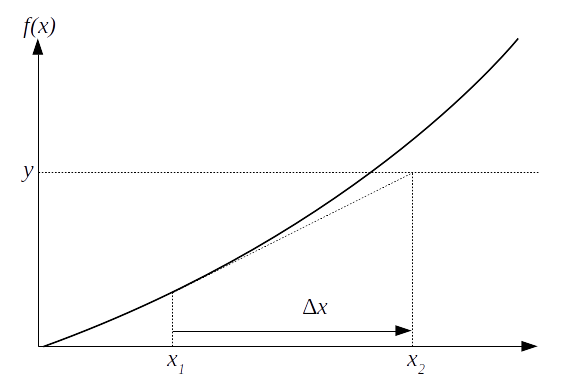
\includegraphics[width=0.8\linewidth]{figures/1d_newton}
\caption{An example iteration step using simple Newton-Rhapson iteration.}\label{fig:1d:newton}
\end{figure}

Newton iteration converges quickly on ``well mannered'' functions that are more or less parabolic in their shape, but there are significant problems when functions show more complicated shapes.

\subsection{ITER1: Modified Newton-Rhapson Iteration}

In many cases, there are hard boundaries above which no solution is possible.  These conditions often occur along with numerically stiff functions like the one shown in Figure \ref{fig:1d:newton:bounded}.  Here the funciton diverges rapidly as it approaches an asymptote.

In many of these cases, the locations of those asymptotes can be known even if the exact solution to the problem is not.  The ITER1 algorithm defined in \pm is a Newton-Rhapston solver modified to respect upper and lower bounds that limit the range over which an algorithm may stray.  If a guess leaves this range, the algorithm halves the step, $\Delta x$, until the new guess is back in range.

In Figure \ref{fig:1d:newton:bounded}, the first iteration produces a guess outside of the upper boundary, so $\Delta x$ is adjusted until the new guess is in-bounds again.  In this example, only one adjustment is necessary, but it could have continued many times.

\begin{figure}
\centering
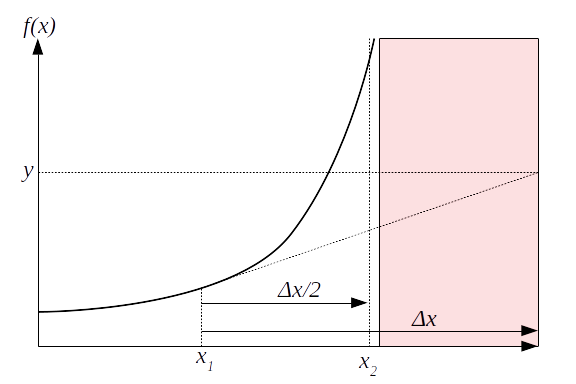
\includegraphics[width = 0.8\linewidth]{figures/1d_newton_bounded}
\caption{An example of an iteration step using the ITER1 method.  The red box represents values beyond the legal solution boundary.}\label{fig:1d:newton:bounded}
\end{figure}

\begin{enumerate}
\item \underline{Given:} a funciton, $f(x)$, a target value, $y$, an initial guess, $x_0$, an acceptable error for $f(x)$, $\epsilon$, and upper and lower limits on $x$,
\item Set the current guess, $x_k$ to $x_0$.
\item Evaluate $f(x_k)$ and $f'(x_k)$. \label{newton:bounded:goto1}
\item If $|y-f(x_k)| < \epsilon$.  If error is small, $x_k$ solves the problem.
\item Calculate a distance to move the guess, $\Delta x = (y - f(x_k))/f'(x_k)$
\item Calculate a new guess $x_{k+1} = x_k + \Delta x$.\label{newton:bounded:goto2}
\item If $x_{k+1}$ is outside the limits, divide $\Delta x$ by 2. Return to step \ref{newton:bounded:goto2}
\item Return to step \ref{newton:bounded:goto1}
\end{enumerate}

This method is quite robust in the sense that it will either converge to an answer or it will toil on infinitely.  Provided the limits on $x$ are well selected, it cannot diverge wildly like the guess in Figure \ref{fig:1d:newton:bounded}.

It should be emphasized, however, that Newton-Rhapson iteration is highly susceptible to infinite cycles when functions are shaped like Figure \ref{fig:1d:newton:cycle}.  This depicts an infinite cycle of guesses that will never converge to a solution.  It could be disregarded as an esoteric curiosity were it not precisely the type of failure that occurs when iterating on properties near phase changes (or near the critical point of a fluid).

\begin{figure}
\centering
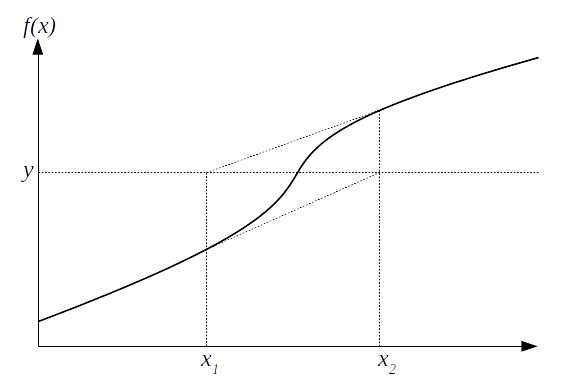
\includegraphics[width = 0.8\linewidth]{figures/1d_newton_cycle}
\caption{An example of an endless cycle using bisection or ITER1.}\label{fig:1d:newton:cycle}
\end{figure}

For this reason, the ITER1 algorithm is relegated to the well behaved curves found in ideal gas properties.  A more sophisticated algorithm is needed for multi-phase properties.  In practice, ITER1 usually converges in three or four iterations to .001\% or better on ideal gas data.  There are some species that use the Shomate equation that have small discontinuities in their specific heat curves.  In extremely rare circumstances, this can cause strange numerical problems when the solution lies very near the discontinuity.

\subsection{An introduction to bisection iteration}

Given that failure to converge can be as bad as crashing, there is some incentive to implement a numerical routine that \emph{must} converge.  In one dimension, the bisection algorithm is an excellent choice when stability is valued over speed.

If upper and lower bounds, $x_a$ and $x_b$ are found so that $f(x_a) < y < f(x_b)$, then any continuous function must have a value somewhere between $x_a$ and $x_b$ such that $f(x) = y$.  If we were to divide the domain in half $x_c = (x_a+x_b)/2$ and evaluate the function there, its value will either be above or below $y$, so one of the two values could be replaced by $x_c$.  In this way, the domain between $x_a$ and $x_b$ is reliably cut in half with every iteration step, no matter how bizarrely $f(x)$ behaves.

This process just has to be repeated until the distance between the upper and lower bounds have shrunk to be so small that the numerical uncertainty is acceptable.  Figure \ref{fig:1d:bisection} shows three steps using this process.  The vertical space occupied by each blue box represents the shrinking uncertainty for the value of $f(x)$ and the horizontal space represents the shrinking uncertainty in $x$.

\begin{figure}
\centering
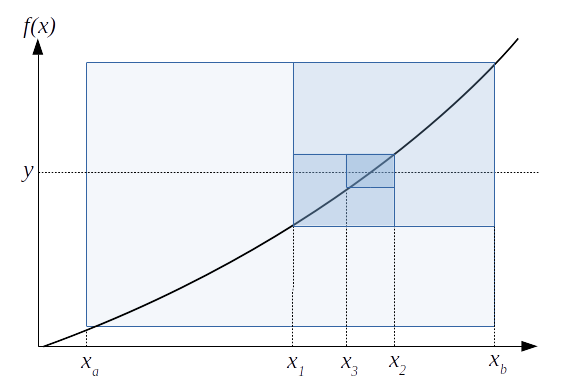
\includegraphics[width = 0.8\linewidth]{figures/1d_bisection}
\caption{An example of three iteration steps using the bisection algorithm.}\label{fig:1d:bisection}
\end{figure}

While Newton iteration might converge in only a few steps, bisection can take tens of steps depending on the ratio of the initial domain and the acceptable error range.  Since the domain is divided by two every time, it is easy to calculate the number of iterations to obtain a certain domain size.
\begin{align}
N = \log_2 \frac{|x_b - x_a|}{\epsilon}
\end{align}
If the initial domain were a temperature range of 0 to 1000 Kelvin, and the acceptable error were .01 Kelvin, 17 iterations are required.  If the acceptable error were tightened to .001 Kelvin, 20 iterations are required!

\subsection{HYBRID1}

It is difficult to walk away from guaranteed convergence even if bisection iteration is very slow.  It would be nice if there were some way to use a Newton-like algorithm that defaulted to a bisection algorithm when things go badly.  The trouble is how to figure out when things are going badly without adding numerically expensive checks.

Like bisection, HYBRID1 begins with upper and lower bounds, $x_a$ and $x_b$, which must bracket a solution.  Unlike bisection, HYRBID1 does not assume that all points in the range are equally likely to be solutions.  Newton iteration is used as much as possible, but (1) the two bounds must always bracket a solution, and (2) no guess should ever widen the bounds.

Each iteration step is allowed to select one of three candidate guesses.  As depicted in Figure \ref{fig:1d:hybrid}, two guesses are generated by performing a Newton iteration step at the upper and lower bounds, and a third bisects the domain.  

\begin{figure}
\centering
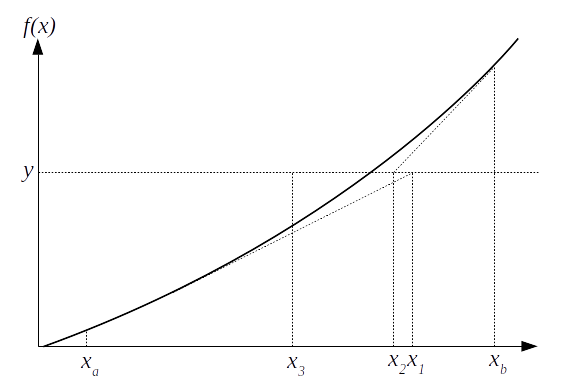
\includegraphics[width = 0.8\linewidth]{figures/1d_hybrid}
\caption{An example of a single iteration step using the HYBRID1 algorithm.}\label{fig:1d:hybrid}
\end{figure}

If either of the Newton iteration steps lie outside of the domain, the bisection candidate is selected.  In this condition, the behavior of the function at the edges of the domain are clearly not reliable indicators for the behavior of the function inside the domain, so they should be disregarded.  This mitigates both the endless cycle shown in Figure \ref{fig:1d:newton:cycle} and the divergence in Figure \ref{fig:1d:newton:bounded}, as well as other common numerical traps.

If all three candidate values lie inside the range between $x_a$ and $x_b$, the middle of the three is selected.  When the two Newton steps lie on opposite sides of the bisection, it is apparent that they disagree enough that they cannot be trusted, so bisection is the safest (and probably the fastest) choice.  This also mitigates certain ways of encountering Figure \ref{fig:1d:newton:cycle}.  When the Newton candidate guesses lie on the same side of the bisection candidate, they agree well enough that the solution is likely to be nearby, like in Figure \ref{fig:1d:hybrid}.

The function and its derivative are only evaluated at the selected candidate value; the other two are left alone.  This description of the process may lead one to imagine that each iteration step requires two function evaluations, but that is not so.  Just like the bisection algorithm, the appropriate upper or lower bound is replaced by the next guess so that the two bounds continue to bracket a solution.  The efficiency of this approach is realized by not discarding the Newton iteration already performed on the other bound.  Only one new function evaluation is necessary per step.

\begin{enumerate}
\item \underline{Given:} a function $f(x)$, a target value, $y$, upper and lower bounds, $x_a$ and $x_b$, and acceptable error bands on $x$, $\epsilon_x$ and $y$, $\epsilon_y$.
\item Evaluate $f(x_a)$, $f'(x_a)$, $f(x_b)$, and $f'(x_b)$.
\item If necessary, swap $x_a$ and $x_b$ so that $f(x_a) < y < f(x_b)$.
\item If $y$ is not between the two function values, throw an error.
\item Calculate three candidate guesses:
    \begin{enumerate}
    \item $x_1 \leftarrow x_a + (y-f(x_a))/f'(x_a)$
    \item $x_2 \leftarrow x_b + (y-f(x_b))/f'(x_b)$
    \item $x_3 \leftarrow (x_a + x_b)/2$
    \end{enumerate}
\item Select a candidate, and store it as $x_c$: \label{1d:hybrid:goto}
    \begin{enumerate}
    \item If either $x_1$ or $x_2$ is outside of $x_a$ and $x_b$, use $x_c \leftarrow x_3$.
    \item Otherwise, set $x_c$ equal to the middle value, $x_c \leftarrow \mathrm{median}(x_1, x_2, x_3)$.
    \end{enumerate}
\item Evaluate $f(x_c)$ and $f'(x_c)$.
\item If $|f(x_c) - y| < \epsilon_y$, $x_c$ solves the problem.
\item If the new guess is less than the target ($f(x_c) < y$),
    \begin{enumerate}
    \item Replace $x_a \leftarrow x_c$, $f(x_a) \leftarrow f(x_c)$, and $f'(x_a) \leftarrow f'(x_c)$
    \item Calculate a new candidate for the lower bound, \\$x_1 \leftarrow x_a + (y-f(x_a))/f'(x_a)$
    \end{enumerate}
\item If the new guess is greater than the target ($f(x_c) > y$),
    \begin{enumerate}
    \item Replace $x_b \leftarrow x_c$, $f(x_b) \leftarrow f(x_c)$, and $f'(x_b) \leftarrow f'(x_c)$
    \item Calculate a new candidate for the upper bound, \\$x_2 \leftarrow x_b + (y-f(x_b))/f'(x_b)$
    \end{enumerate}
\item Calculate a new bisection candidate, $x_3 \leftarrow (x_a + x_b)/2$.
\item If the domain is narrow, $|x_b - x_a| < 2\epsilon_x$, then the problem is solved by $x_3$.
\item Return to step \ref{1d:hybrid:goto}
\end{enumerate}

The reader is encouraged to walk through the algorithm graphically using Figure \ref{fig:1d:hybrid}.  It should be apparent that the second iteration step will be a bisection step even though a second Newton iteration should be more expedient.  However, the third step arrives remarkably close to the solution.  In this way, the cautious approach employed in HYBRID1 carries a cost when employed on well behaved functions.

In practice, HYBRID1 usually converges with one or two extra function evaluations compared with ITER1 on well behaved functions like those found in ideal gas properties.  However, in multi-phase systems, ITER1 often fails to converge, and HYRID1 dramatically outperforms traditional bisection.  


\section{Considerations for Array Support}

\end{document}
